\documentclass[10pt]{beamer}
\usetheme{Celestia}

\usepackage[utf8]{inputenc}
\usepackage[T1]{fontenc}
\usepackage{booktabs}
\usepackage{tikz}
\usetikzlibrary{positioning}

\title{Photogallery, un'applicazione a microservizi}
\subtitle{Progetto per il corso di Sistemi Distribuiti e Cloud Computing}
\author{Matteo Orlando 0382170}
\institute{Università degli studi di Roma Tor Vergata}
%\date{\today}

\begin{document}

\maketitle

\begin{frame}{Indice}
  \tableofcontents
\end{frame}

\section{Introduzione}
\begin{frame}{Obiettivo}
Lo scopo di questo progetto è implementare un sistema di notifiche per gallerie fotografiche realizzato come applicazione a microservizi in Go.
\hspace{2cm}
 \begin{columns}[T]
 	\begin{column}{0.48\textwidth}
      \textbf{Requisiti non funzionali}
      \begin{itemize}
        \item Implementazione in Go
        \item Comunicazione tra i servizi tramite gRPC
        \item Il sistema deve essere scalabile e adeguatamente testato
        \item Deploy tramite Docker su EC2
      \end{itemize}
    \end{column}
    \begin{column}{0.48\textwidth}
      \textbf{Requisiti funzionali}
      \begin{itemize}
        \item Registrazione di utenti e moderatori    
        \item Gestione delle gallerie da parte dei moderatori    
        \item Caricamento di foto nelle gallerie    
        \item Notifica ai membri della galleria dei nuovi caricamenti
      \end{itemize}
    \end{column}
  \end{columns}
\end{frame}

\begin{frame}{Tecnologie adottate}
\begin{figure}    
\centering    
	\begin{tabular}{cccc}        
		
\includegraphics[width=0.20\textwidth]{grpc.png} &
		
\includegraphics[width=0.20\textwidth]{postgres.png} &       
		
\includegraphics[width=0.20\textwidth]{docker.png} &  
		
\includegraphics[width=0.20\textwidth]{aws.png} 
		\\[0.6cm]  
		
\includegraphics[width=0.20\textwidth]{rabbitmq.png} &    
		
\includegraphics[width=0.20\textwidth]{redis.png} & 
		
\includegraphics[width=0.20\textwidth]{minio.png} &        		
		
\includegraphics[width=0.20\textwidth]{react.png}    
	\end{tabular}
\end{figure}
\end{frame}


\begin{frame}{Pattern adottati}
\begin{table}
\small
\begin{tabular}{@{}p{3.3cm}p{5.8cm}@{}}
\toprule
\textbf{Pattern} & \textbf{Dove} \\
\midrule
CQRS & Gallery Service: separa scrittura e lettura \\
Circuit Breaker & Upload $\rightarrow$ Gallery: resilienza a fallimenti \\
Database per Service & Ogni microservizio che necessita persistenza \\
Flux & Frontend: flusso unidirezionale per gestire lo stato\\
\bottomrule
\end{tabular}
\end{table}
\end{frame}


\begin{frame}{Architettura}
\begin{figure}[t]
\centering
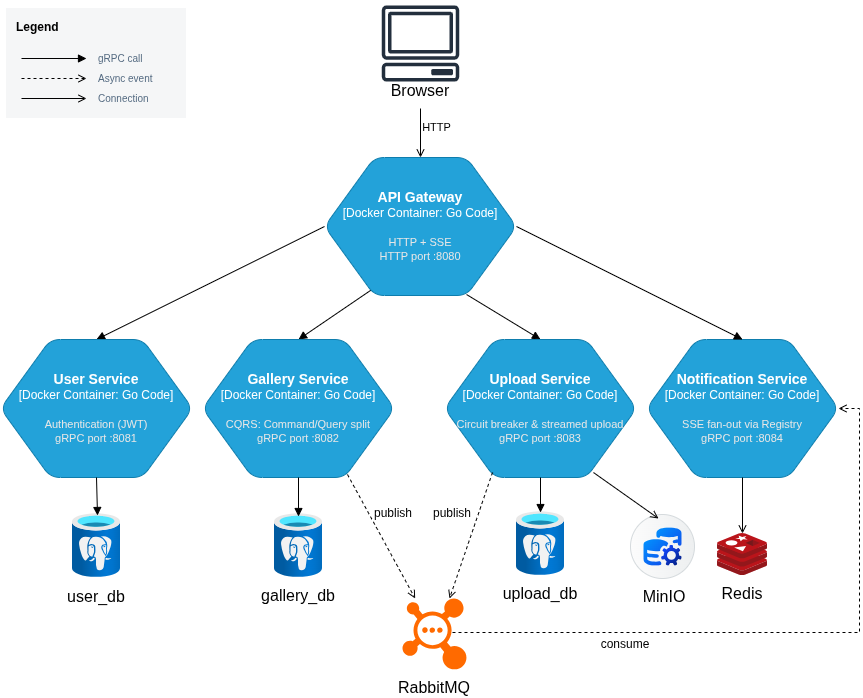
\includegraphics[width=\textwidth, height=0.9\textheight, keepaspectratio]{architettura.png}
\end{figure} 
\end{frame}

\section{Implementazione}
\begin{frame}{Framework e strumenti utilizzati}
\begin{table}
\small
\begin{tabular}{@{}p{3cm}p{6.1cm}@{}}
\toprule
\textbf{Framework} & \textbf{Ruolo} \\
\midrule
Buf & Generazione codice RPC \\
GORM & ORM per accesso a PostgreSQL \\
GoMock & Mock generati per unit test \\
grpc-gateway & Reverse proxy HTTP $\rightarrow$ gRPC \\
Gin & Route non-unary: upload, SSE \\
\bottomrule
\end{tabular}
\end{table}
\end{frame}

\begin{frame}{CQRS nel Gallery Service}
\begin{columns}[T]
\begin{column}{0.48\textwidth}
\textbf{Comandi (write)}
\begin{itemize}
    \item CommandRepository
    \item Logica di business in CommandService
    \item Verifica autorizzazione prima di modificare lo stato
    \item Pubblicazione asincrona su RabbitMQ dopo il commit
\end{itemize}
\end{column}

\begin{column}{0.48\textwidth}
\textbf{Query (read)}
\begin{itemize}
    \item QueryRepository
    \item Logica di business in QueryService
    \item Operazioni idempotenti
    \item Recupero dati ottimizzato per la lettura
\end{itemize}
\end{column}
\end{columns}
\end{frame}

\begin{frame}{Circuit breaker}
\begin{columns}[T]
\begin{column}{0.45\textwidth}
\centering
	\begin{itemize}    		
    		\item Tre stati: \textbf{CLOSED}, \textbf{OPEN}, \textbf{HALF-OPEN}
    		\item Mutex garantisce una sola probe alla volta in HALF-OPEN
    		\item Gestisce i fallimenti senza bloccare le richieste sincrone
     \end{itemize}
\end{column}     
\begin{column}{0.55\textwidth}
\centering
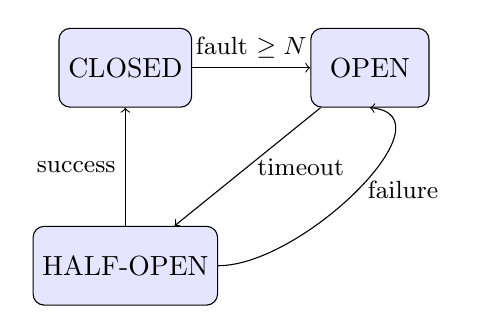
\begin{tikzpicture}[node distance=1.5cm, auto,
    state/.style={rectangle, rounded corners, draw, fill=blue!10, minimum width=1.5cm, minimum height=1cm}]
    \node[state] (closed) {CLOSED};
    \node[state, right=of closed] (open) {OPEN};
    \node[state, below=of closed] (half) {HALF-OPEN};

    \draw[->] (closed) -- node[above, font=\small]{fault $\geq N$} (open);
    \draw[->] (open) -- node[right, font=\small]{timeout} (half);
    \draw[->] (half) -- node[left, font=\small]{success} (closed);
    \draw[->] (half.east) to[out=0,in=-5,looseness=1] node[right, font=\small]{failure} (open.south);
\end{tikzpicture}
\end{column}     
\end{columns}
\end{frame}


\begin{frame}{Distribuzione notifiche}
\centering
	\begin{itemize}
   	\item L'evento viene pubblicato su RabbitMQ in una goroutine in background, dopo il commit della transazione
    \item Il Notification Service consuma l'evento in modo asincrono e lo trasforma in una notifica per gli utenti interessati
    \item Redis Pub/Sub propaga la notifica a tutte le repliche del Notification Service
   		\item Ogni replica attraverso il registro in memoria inoltra la notifica ai propri client
     \end{itemize}
 \vspace{0.3cm}
\centering
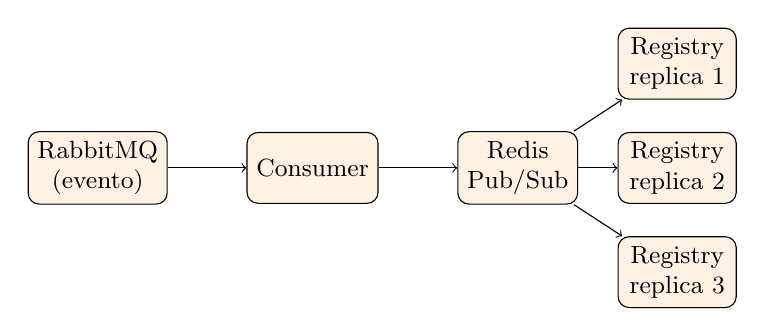
\begin{tikzpicture}[node distance=1.0cm, auto,
    box/.style={rectangle, draw, rounded corners, fill=orange!10, minimum height=0.9cm, minimum width=1.5cm, align=center, font=\small}]
    \node[box] (mq) {RabbitMQ\\(evento)};
    \node[box, right=of mq] (consumer) {Consumer};
    \node[box, right=of consumer] (redis) {Redis\\Pub/Sub};
    \node[box, above right=0.4cm and 0.5cm of redis] (r1) {Registry\\replica 1};
    \node[box, right=0.5cm of redis] (r2) {Registry\\replica 2};
    \node[box, below right=0.4cm and 0.5cm of redis] (r3) {Registry\\replica 3};

    \draw[->] (mq) -- (consumer);
    \draw[->] (consumer) -- (redis);
    \draw[->] (redis) -- (r1);
    \draw[->] (redis) -- (r2);
    \draw[->] (redis) -- (r3);
\end{tikzpicture}
\end{frame}

\begin{frame}{Metodologia di testing}
\begin{itemize}
    \item \textbf{Unit test}: dipendenze esterne mockate con GoMock
    \item \textbf{Test di integrazione}: client black-box contro lo stack HTTP reale
    \item \textbf{Load test}: generano carico concorrente pesato verso il Gateway, misurando throughput, latenza e tasso di errore.
\end{itemize}
\end{frame}


\section{Risultati}
\begin{frame}{Load test: 1 replica vs 3 repliche}
\begin{table}
\centering
\small
\begin{tabular}{lcccc}
\toprule
\textbf{Servizio} & \textbf{Repliche} & \textbf{Throughput} & \textbf{Latenza (min/media/max)} & \textbf{Errori} \\
\midrule
Gallery  & 1 & 44.0 req/s  & 106.30 / 137.04 / 1144.52 ms & 0\% \\
Gallery  & 3 & 69.3 req/s  & 107.42 / 140.54 / 825.89 ms  & 0\% \\
\midrule
Upload   & 1 & 107.0 req/s & 106.03 / 184.30 / 1229.10 ms & 63.8\% \\
Upload   & 3 & 111.7 req/s & 106.00 / 182.45 / 1232.62 ms & 47.9\% \\
\bottomrule
\end{tabular}
\end{table}
\end{frame}

\begin{frame}{Limiti}
\begin{itemize}
    \item \textbf{Pubblicazione eventi non atomica}: un crash intermedio può far perdere un evento
    \item \textbf{Registry in memoria}: lo stato delle connessioni SSE va ricostruito ad ogni riconnessione
    \item \textbf{Single point of failure}: RabbitMQ, Redis e le tre istanze PostgreSQL non sono replicate
\end{itemize}
\end{frame}

\begin{frame}{Compromessi}
	\begin{itemize}
	    \item \textbf{Ridondanza RabbitMQ + Redis}: ogni replica del Notification Service deve riapplicare localmente il filtraggio degli eventi ricevuti via Pub/Sub
        \item \textbf{Deployment single-host}: Docker Compose su una singola istanza EC2 semplifica la riproducibilità, ma non consente una vera distribuzione multi-host né una disponibilità da ambiente di produzione
    \item \textbf{Robustezza dei load test}: i risultati dipendono da dimensioni dell'istanza, numero di repliche e singola esecuzione
	\end{itemize}
\end{frame}

\section{Conclusioni}
\begin{frame}{Conclusioni}
\begin{itemize}
    \item CQRS permette la separazione tra logica di scrittura e di lettura, testing isolato dei due percorsi
    \item Circuit Breaker garantisce resilienza verso i malfunzionamenti del Gallery Service
    \item RabbitMQ e Redis Pub/Sub permettono la corretta distribuzione delle notifiche
    \item Suite di test permette di verificare la correttezza funzionale e il comportamento sotto scalabilità/guasto
    \item Sviluppi futuri: atomicità tra scrittura e pubblicazione eventi, separazione fisica del modello di lettura, migrazione a Kubernetes, monitoring/logging distribuito
\end{itemize}
\end{frame}

\begin{frame}
  \centering
  \Large Grazie per l'attenzione
\end{frame}

\end{document}
